\chapter{Problem \& Algorithm Design}
\label{chp:algorithm}

\section{Why Existing Methods Fall Short}

The two methods this work builds on \hlnotein{each steer toward}{The grammar is weird. just say
The two methods, mentioning what two again. both demostrate sucessfuly navigation in the paper} a single light, 
but neither is enough for the navigation we \hlnotein{are after}{Don't write it like stuff we are after
write it the two methods fail}. The bearing points straight at the source and works well in open space, 
yet it has no memory of where the light is: the moment an obstacle blocks the line of sight, the drone 
is \hlnotein{left without a heading and cannot find its way around.}{Write it like this. Once the obstacle blocks
the line of sight, the drone immediately lose the signal and cannot determine the light direction. Thus, it loses
the direction to fine the way toward the light.} Following the light gradient with a single photodiode, 
as in prior work~\cite{huang2026lta}, \hlnotein{fares no better}{Write it more readable. the light gradient
approach also fail in tracking the light when it encounter a obstacle. }, since one sensor must infer the gradient 
from how its signal changes as the drone moves, which is slow and easily confused \hlnote{by noise.}{hmm im not really convinced
is the gradient really fail? i thought we use gradient to pull it away.}

\hlnotein{We study}{it jump directly into the simulation setup too fast. We need to first talk about why dont we
directly do the experiment in real-world to test it? there is multiple reason we can talk about. first, 
the real-world test will have ambient light noise. to first get rid of it we test it in simulation.
second, the simulation give fast repetitive experiment. again mention that here again to bridge reader easier.
} these methods in a Webots simulation that recreates the navigation task,
as Figure~\ref{fig:sim-setup} shows. The scene places a light source over the floor, 
an obstacle pillar in the path, and the drone to one side, so that the line of sight from 
the drone to the light is blocked \hlnotein{unless the drone first routes around the pillar.}{I dont feel necessary to mention
routes around the pillar here. just mentioned it will be blocked is enough.}
Every controller we compare in this chapter, the bearing-only and gradient-only baselines as well 
as the \hlnotein{fused controller}{Here the fused controller just pop out. you can mentioned we have our improved 
controller at the start. but dont bring up the detail term. just say. we tested A and B from Huang. and we show that they
all fail. and we further demonstrate our approach, which do A + B. works. you can mentioned a bit A + B here but dont jump
into detail.}, flies in this same scene from the same start position toward the same beacon, 
with identical sensing and flight settings, so that the only difference between the runs is the navigation 
method itself. The same environment also underlies the experiments of Chapter~\ref{chp:obstacle}.

\begin{figure}[h]
    \centering
    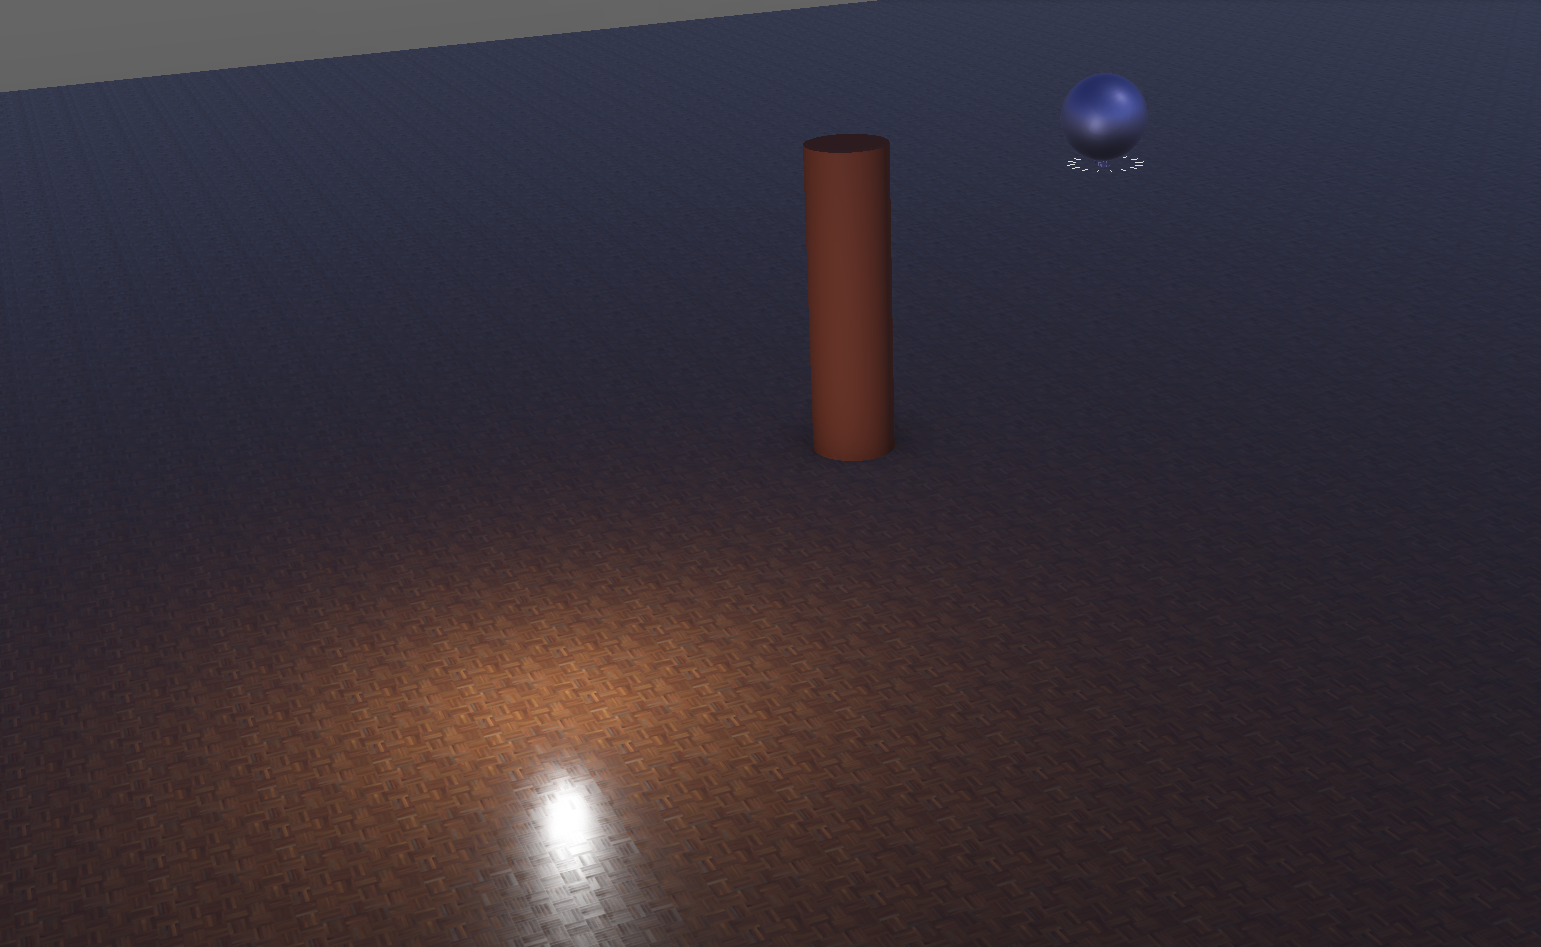
\includegraphics[width=0.6\textwidth]{figures/simulation_setup.png}
    \caption{The simulated test environment in Webots: a light source casting its pool of light on the floor, an obstacle pillar, and the drone approaching from one side.}
    \label{fig:sim-setup}
\end{figure}

In simulation, a bearing-only controller drives toward the light but, having no memory of the field,
cannot plan a way around the obstacle in its path and collides with the pillar, 
as Figure~\ref{fig:bearing-fail} \hlnotein{shows}{Its a long sentence. try to split it can talk
about each sentence more detail}. The collision is already a failure: on a real platform such 
an impact could damage the drone or the \hlnotein{obstacle}{BTW, I do test it myself in the simulation and see it crash
sometimes. but here in the graph it looks like it pass the obstacle? probably we need to make
some postprocess to make it mroe clear. should not be the graph show here}.

\begin{figure}[h]
    \centering
    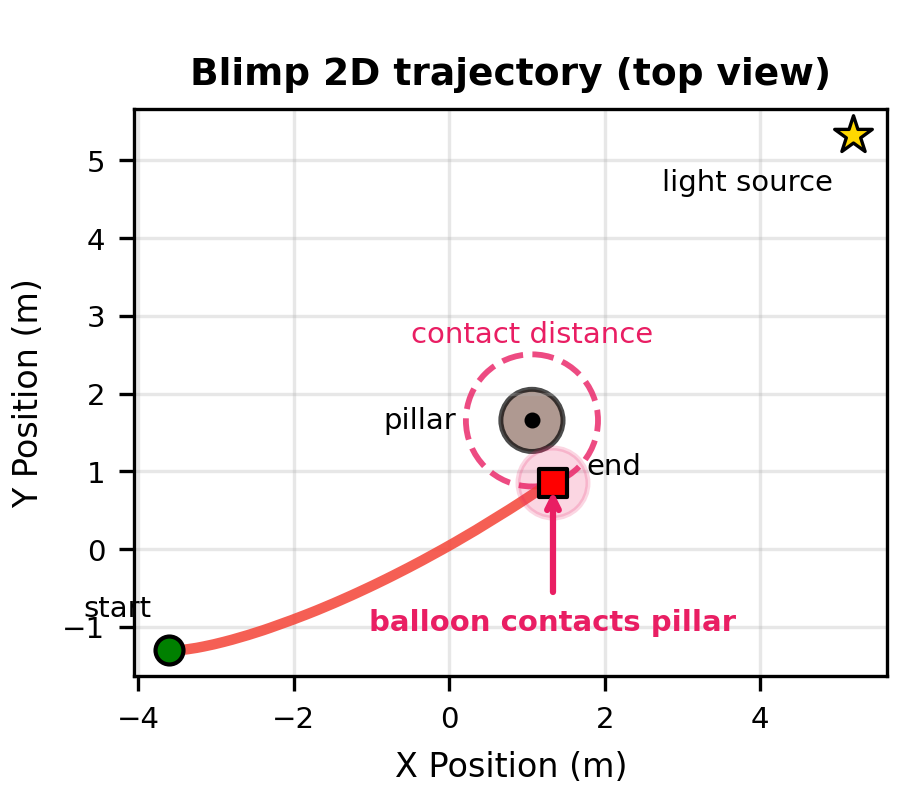
\includegraphics[width=0.6\textwidth]{figures/bearing_only_sim/blimp_trajectory_2d.png}
    \caption{Top-down trajectory in simulation: the bearing-only controller drives into the obstacle and cannot circle it cleanly, having no memory of the field to route around it.}
    \label{fig:bearing-fail}
\end{figure}

The single-photodiode gradient method struggles in 
the same setting: because it can only sense the gradient 
by moving, it follows a slow, wandering path that stalls 
at the obstacle rather than driving cleanly toward the source,
as Figure~\ref{fig:gradient-fail} \hlnote{shows}{This is good! explain a bit more
why it stall? What i understand is that the gradient will pull it away.}. Neither method, moreover, 
has any notion of more than one beacon, so reaching several lights 
in turn is out of reach from the start.

\begin{figure}[h]
    \centering
    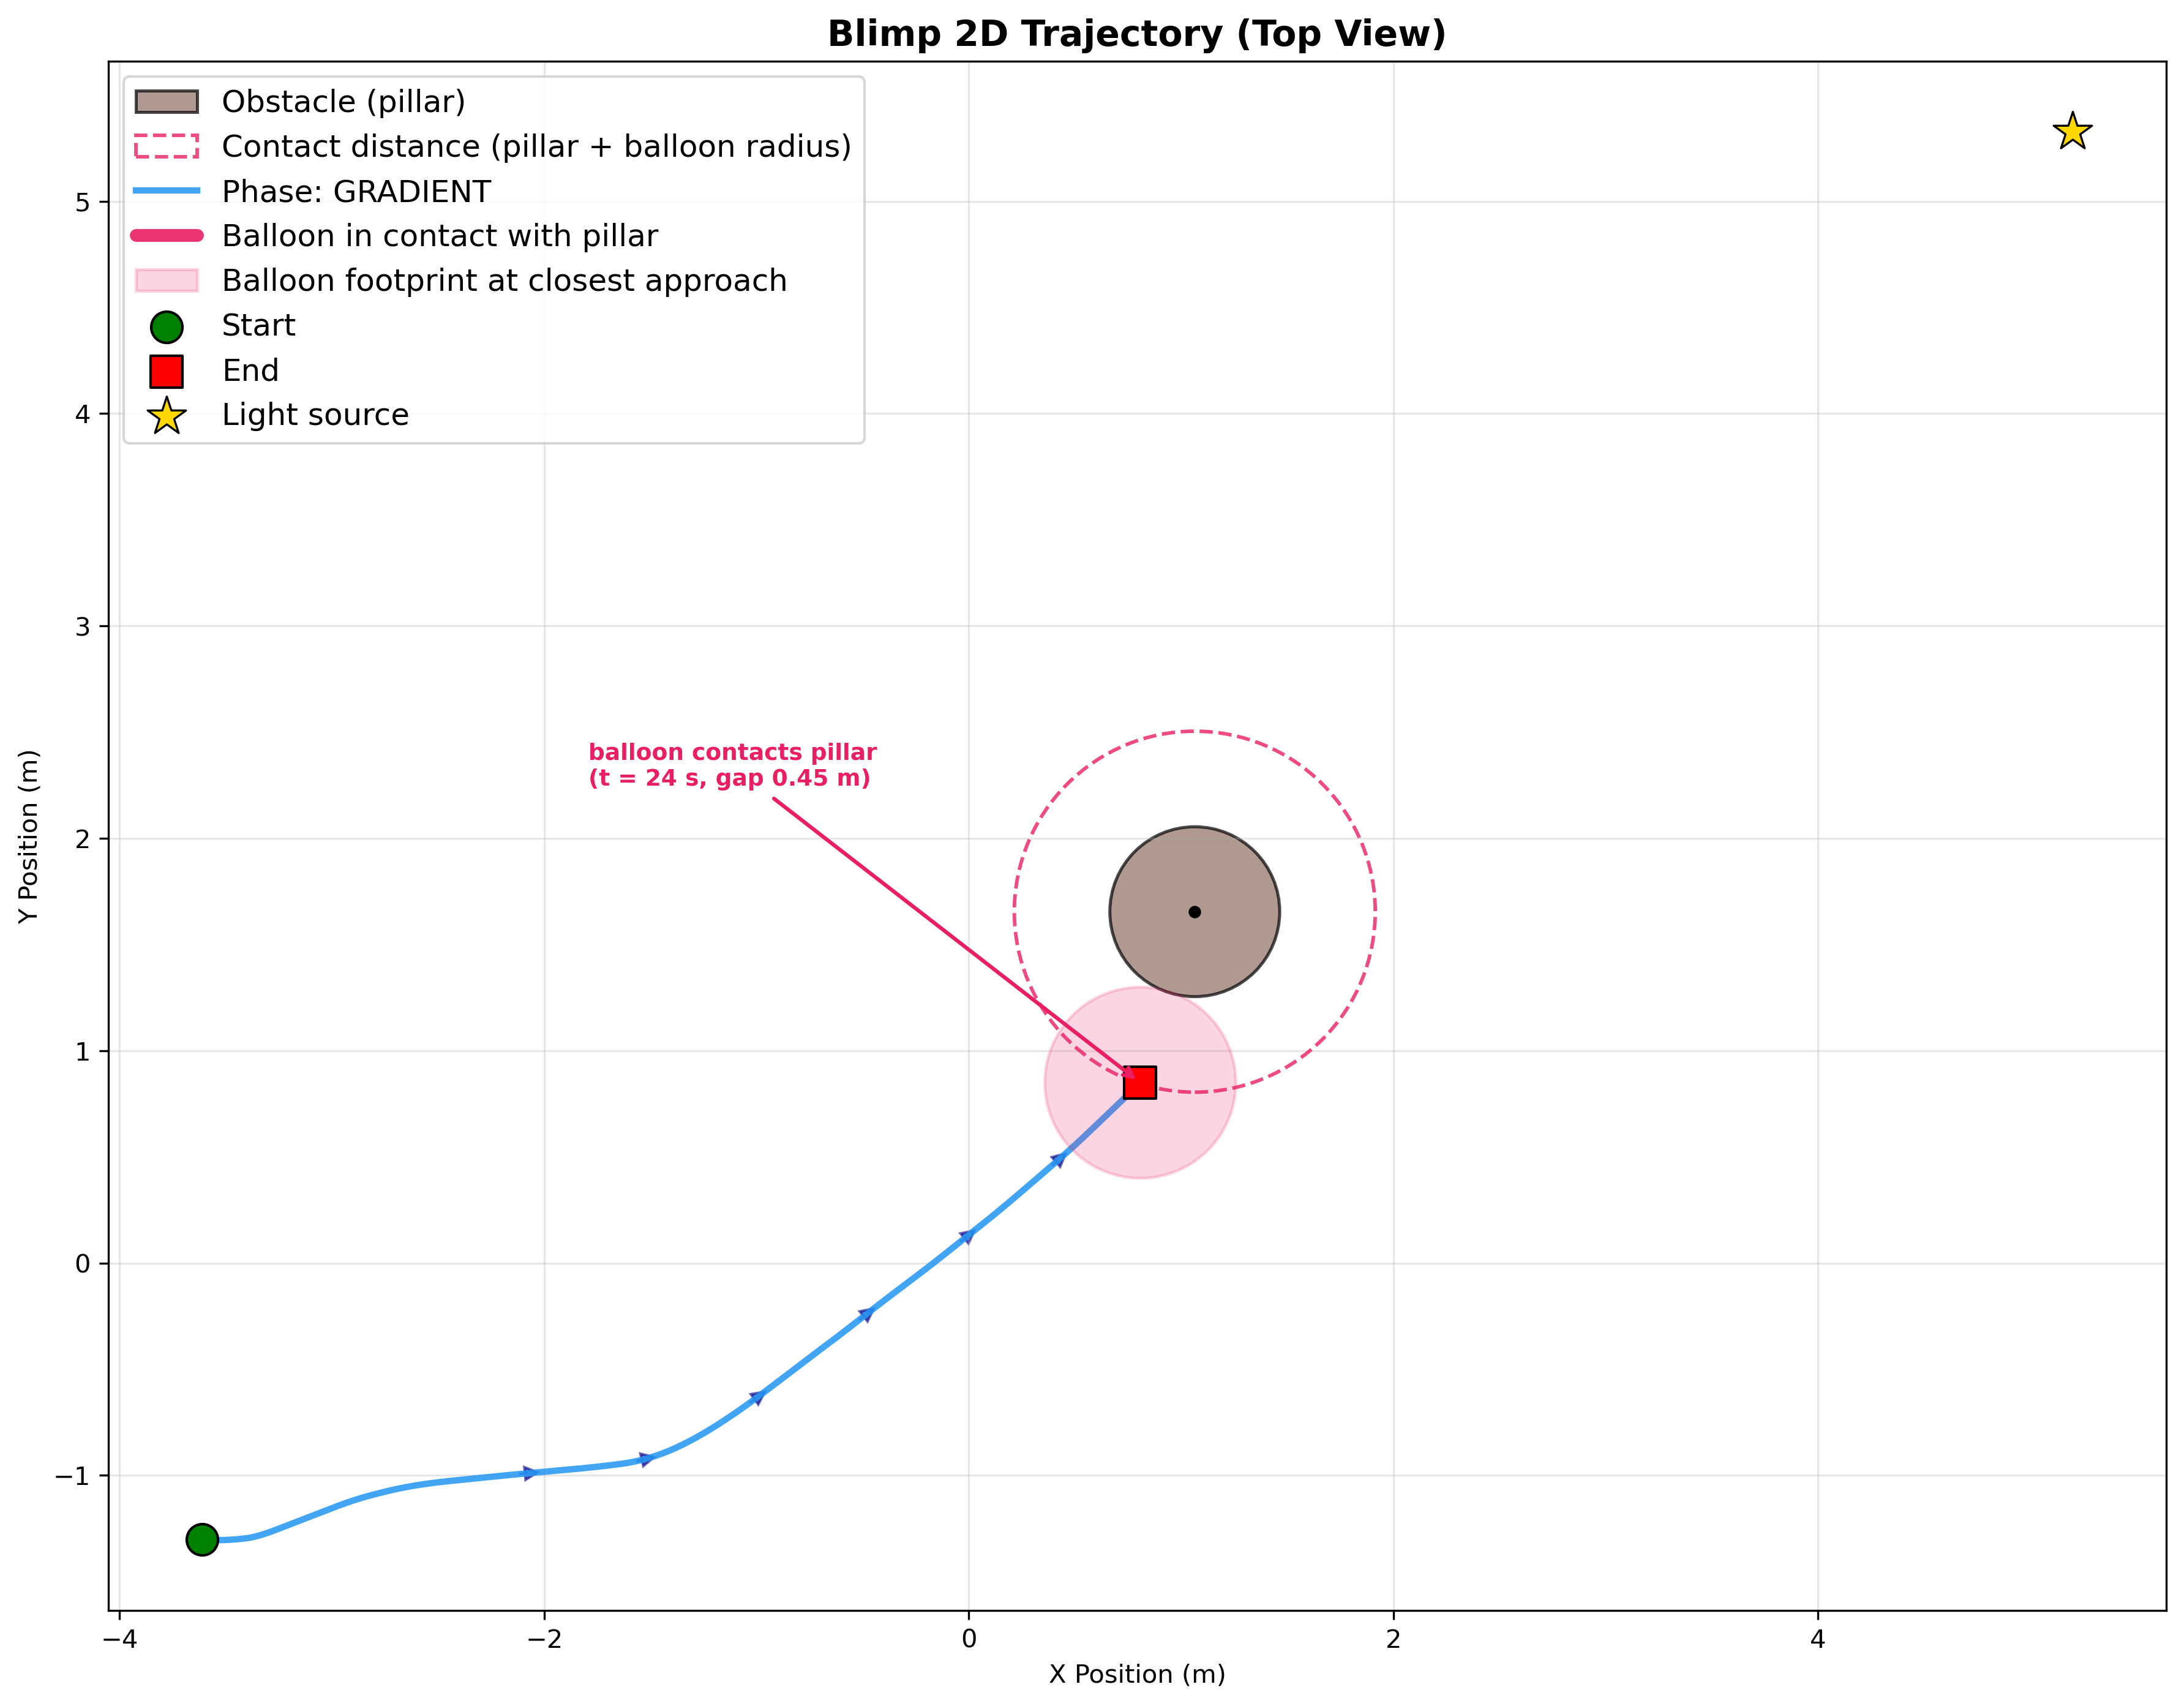
\includegraphics[width=0.6\textwidth]{figures/gradient_only_sim/blimp_trajectory_2d.png}
    \caption{Top-down trajectory in simulation: single-photodiode gradient ascent wanders and stalls at the obstacle, never reaching the light source.}
    \label{fig:gradient-fail}
\end{figure}

These shortcomings set \hlnote{the agenda for the rest of this chapter:}{For my preference
this sounds weird. i would go something like this. As demonstrated, the method proposed
by Huang encounter these shortcomings with both approach. This bring up the center problem in this
research. When there is a simple obstacle in the scene. How can we avoid the obstacle without introducing
extra sensor and complicated algorithm.} 
we develop a controller that fuses the two signals, estimates the
gradient from all eight photodiodes rather than one, and remembers
the light field in a map, so that it can route around \hlnotein{obstacles}{There is no
Why you come up with this. what do you see from the previous experiment for you to bring this up?
We need to bring up both pros and cons and then say that combining it is a good idea.} 
and visit multiple beacons. Its positive results are presented in 
Chapter~\ref{chp:obstacle}.

\section{System Overview}

To guide the drone toward a light beacon, we combine two inputs, both obtained from the same 
photodiode array. The first is a bearing angle that points straight at the source, which gives 
the controller an immediate heading whenever the beacon is in view. The second is a gradient direction, 
read from a map of the light field that the drone builds as it flies; this map records where the light is
stronger, so it stays useful even when the drone can no longer see the beacon directly.

Neither input is enough on its own. As the previous section showed, the bearing is fast but has no memory,
while the gradient is robust but only becomes available once the drone has built up a usable map. 
y combining them we get the best of both: the controller reacts quickly while the beacon is visible, 
yet keeps moving through a brief loss of signal by leaning on the map it has already \hlnotein{built}{this two paragraph
should be put before this}.

\hlnotein{Each update}{we move previous two more up. thus this need to rewrite. we should write it somthing like this.
Our system is aim to tackle a environment like this. in indoor environment where there is multiple
clusttering small obstacle. can we use single light for drone to navigate toward the light while having the 
ability to autonomously avoide the obstacle? and then with this task in mind. we need to achieve two thing. the 
drone need to move toward light efficiently enough -> means we need to use bearing. but also the obstacle avoidance
-> gradient. However, this bring up the problem. when should use use which. and then we bring it up there is a system design
with the state machine control} follows the same steps. \hlnotein{First, the per-sensor}{Lets try to make it more abstract.
This is an example. First the drone alway estimate the light direction using multiple photodiode weighting which we called bearing angle
. In the meanwhile, we collect the light intensity overtime and store them in a map. Where we further utilize this map
for gradient guidance algorithm. However, when there is two target from two algorithm, which one should we use ?
While instead of fully trust either, we propose a fusion model to combined the two} light signals of 
Section~\ref{sec:lightsignal} are turned into a bearing estimate and added to the light map. 
Then the local gradient is read from the map, and the bearing and gradient are merged into a single
target heading. A state machine decides how much to trust each input from the current signal
strength and map coverage, and walks the drone through search, alignment, approach and recovery
phases for each beacon in a multi-target mission, as summarised in Figure~\ref{fig:controller-overview}. The
controller finally outputs a target heading and a forward speed, which are passed to the drone's
own flight controller.

\begin{figure}[h]
    \centering
    \resizebox{\textwidth}{!}{%
    \begin{tikzpicture}[
        >=Latex,
        box/.style={draw, rounded corners, align=center, minimum height=9mm,
                    inner sep=4pt, font=\small}
    ]
        \node[box] (pd)      at (0,0)      {Photodiode\\array};
        \node[box] (bearing) at (2.7,1.0)  {Bearing};
        \node[box] (map)     at (2.7,-1.0) {Light map};
        \node[box] (grad)    at (5.0,-1.0) {Gradient};
        \node[box] (fuse)    at (7.6,0)    {Fusion and\\state machine};
        \node[box] (out)     at (10.4,0)   {Heading and\\speed};
        \node[box] (fc)      at (12.9,0)   {Flight\\controller};

        \draw[->] (pd) -| (bearing);
        \draw[->] (pd) -| (map);
        \draw[->] (map) -- (grad);
        \draw[->] (bearing) -| (fuse);
        \draw[->] (grad) -| (fuse);
        \draw[->] (fuse) -- (out);
        \draw[->] (out) -- (fc);
    \end{tikzpicture}}
    \caption{Overview of the fused navigation controller. The photodiode array feeds both a bearing estimate and a light map; the gradient is read from the map; the fusion and state-machine stage merges the bearing and gradient into a target heading and forward speed, which are passed to the drone's flight controller.}
    \label{fig:controller-overview}
\end{figure}

\section{Bearing Angle}

The first input to the controller is a bearing angle that points from the drone toward 
the light source. We obtain it from the bearing estimation algorithm of prior work 
by Harry Huang~\cite{huang2026lta}, which combines the relative light-signal magnitudes measured
 across the photodiode ring into a single direction; the full derivation is given in Section~\ref{sec:bearing}. This
gives the controller an immediate sense of where the beacon lies, without having to explore the environment first.

\hlnotein{Not every bearing can be trusted}{again try to elaborate more
try to do like this. However, Not ever bearing angle estimatione is accurate. For example, when the weighting 
is all zero, which represents there is no signal strength measured, the bearing angle will be random number instead of
pointing towards the light. Thus we need a value to score the confidence of the bearing estimation}, so each one comes 
with a measure of signal strength. We only act on a bearing when its strength is above a minimum threshold, 
which keeps the controller from chasing a heading that is really just noise from a weak, distant or absent 
beacon. \hlnotein{The bearings that do pass this check are then smoothed over time}{talk about why we smooth it. because it 
jitter still due not noise or due to sudden change is not favorable. there are multiple reasons why we want to smooth
it. but talk about it first and then speak about the smoothing method} with an exponential moving average, 
so that a single noisy frame does not cause an abrupt change of heading before the bearing reaches the fusion 
stage and the state machine. The update is
\begin{equation}
\hat{\psi}_B \leftarrow \hat{\psi}_B + (1-\beta)\,\Delta,
\label{eq:bearing-filter}
\end{equation}
where $\Delta$ is the wrapped angular difference between the new bearing and the current estimate $\hat{\psi}_B$, and $\beta$ controls how much of the history is kept.

\section{Multi-Beacon Traversal}

\hlnotein{A mission can involve several beacons, each modulated at its own frequency.}{It should be like this. A common application
might require several target anchors. To achieve this, we modulated multiple lights with different frequency} The drone 
senses all of them at the same time but visits them one after \hlnotein{another}{should be something like this. However,
When multiple light in the same environment. The drone can sense multiple light in the same time. To seperate each setpoint
for drone to traverse the targets accordingly we need to do the frequency analysis}. A single frequency analysis 
of the photodiode signal already contains every beacon's peak at once, so 
the sensing is fully parallel, as we show in Section~\ref{sec:freq-separation}; the controller then
picks one beacon as its current target, flies to it, and on arrival selects the next, so the \hlnotein{traversal 
itself is sequential.}{This is an example that passive term makes it not strong enough. It should be so we can traverse target.
Not something can \textit{traveral}}

What makes this possible is the frequency analysis at the heart of the sensing pipeline, introduced 
in Section~\ref{sec:lightsignal}. Each beacon blinks at its own rate, so taking an 
FFT of a photodiode's signal decomposes that signal into its frequency components, 
and every beacon then shows up as a separate peak at its own modulation frequency whose height reflects how 
strongly that beacon is seen. Because a single recording already contains every beacon's peak, we 
can read all of them from the same data rather than attending to one beacon at a time.

We must, however, choose these frequencies with care, because we modulate each beacon by switching its 
light on and off, which produces a square wave that carries strong energy not only at its 
own frequency but also at its odd harmonics~\cite{oppenheim1999dsp}. The frequency analysis 
itself separates a fundamental from its harmonics cleanly, since they fall in different bins; the 
danger is that if one beacon's frequency coincides with a harmonic of another, that harmonic deposits
energy in the wrong beacon's bin and the two become hard to tell apart. We therefore \hlnotein{space the modulation 
frequencies so that none lands on another's harmonics}{We therefore pick frequencies set that has minimum overlapping both
in their main frequency and the hormonic}, \hlnotein{a scheme we arrived at through a set of simple static
experiments on the Teensy platform.}{We first use a static board to retreive the best frequency pair.}

\section{Light Intensity Map}

As the drone flies, we build a spatial map of the light field that serves as the basis for
gradient-based \hlnotein{navigation.}{Again, try to rewrite this. first we need to talk about why. Thus it should be 
somthing like. Apart from the Bearing Angle Algorithm, we need to record the data overtime for gradient estimation.
Since we care more about the spacial distribution (talk about why), we make grid map.} We turn the environment into a regular grid, and
each cell records the strength of the light signal we measure as the drone
passes through it, \hlnotein{indexed by the drone's estimated position in a fixed world frame.}{I would skip explaining this}
\hlnotein{Using a grid keeps the map compact:}{Why we need to make it compact? lets reverse the later senteces.
First talk about the drift and what problem it will cause on the map. and then we try to update the latest in each map.} instead of storing every individual measurement,
we combine all the readings that fall within the same cell into one representative value,
so the size of the map depends on the area covered rather than on how long the drone has been 
flying. Because each reading is filed under the drone's estimated position, the map is only as trustworthy
as that estimate: drift in the position estimate would smear the recorded field across neighbouring cells and
blur the gradient we read from it. We assume the drone's onboard position estimate is accurate enough over the 
course of a mission for this smearing to stay small. We also limit how far the drift can accumulate: the map is 
not kept for the whole mission but reset whenever the drone switches from one beacon to the next, so it is always 
rebuilt afresh for the current beacon and any position error built up while chasing the previous one is discarded 
with the old map. 

The value we keep in a cell is the strongest light signal measured across the photodiode array 
at that location, using the per-sensor light signal defined in Section~\ref{sec:lightsignal}. When the drone
revisits a cell, we do not overwrite its value but blend it with the new measurement through an \hlnotein{exponential 
moving average,}{Again if you want to mentioned the moving average. its better to mentioned why? the reason can 
be that sometimes we observe some noise. but if there is no concrete reason. just skip it.}
\begin{equation}
I_{\text{cell}} \leftarrow \alpha\,I_{\text{cell}} + (1-\alpha)\,I_{\text{new}},
\label{eq:map-blend}
\end{equation}
which smooths out the short-lived fluctuations that occur as we sample the same location again over time. 
The smoothing factor $\alpha$ is set by default to weight the stored and new values equally; 
lowering it makes a cell follow new measurements more closely at the cost of more noise, 
while raising it gives a smoother but slower-adapting map.

The map therefore approximates a scalar field that rises 
toward the source, since the measured signal grows as the drone approaches the beacon, 
and this gives the drone a spatial memory of the light that the reactive bearing alone lacks. 
\hlnotein{Turning the field into a heading is the job of the gradient estimator described next.}{No, write it more like this
With a proximity to the light intensity map, we can then perform gradient estimation on this map. instead saying some task
is left.}

\section{Gradient Estimation}

\hlnotein{Gradient estimation gives the drone the direction it follows across the light map.}{The bearing angle
also gives direction. what is the difference. we need to pinpoint it precise here.}
Prior work inferred this direction from a single photodiode~\cite{huang2026lta}, reading the 
gradient from how that sensor's signal changed as the drone moved, which is slow because the 
drone must \hlnotein{keep moving to sense anything}{keep moving to collect the intensity data. not sensing 
anything}, \hlnotein{and fragile because one sensor sees the source only 
when it happens to face it.}{Should be, this approach can be fragile since it needs to make sure the
photodiode is facing the light target} The eight-photodiode ring avoids both issues: whichever way the drone 
is yawed at least one sensor faces the source, so its orientation no longer blinds the measurement,
and each location is captured directly rather than inferred \hlnotein{from motion.}{So we are doing 
difference, instead using 1 we are using 8. you point out the problem but the senstence end like we did not 
use it as a solution. so end it like. thus, we use 8 photodiode since it is less prone to the occlusion from
diffrence angle.}

\hlnotein{We estimate the gradient by fitting a plane to the map.}{start it like this. With the collected
light intensity map. we can thus estimate which direction the drone should mobe to increasing the 
light intensity fastest (something like this). To do this. we estimate the gradient direction
using the intensity map. For each cell in the intensity map} To the cells $\{(x_i, y_i, I_i)\}$ near 
the drone's current position we fit $I(x,y) = a x + b y + c$ by weighted least squares, weighting each 
cell by the inverse square of its distance to the drone so that nearer cells count for more, and we
take the gradient as $\mathbf{g} = (a, b)$; the controller steers along $\mathbf{g}$ whenever it 
navigates by the map. The same fit reports how \hlnotein{well the cells agree with the plane, through a weighted
coefficient of determination}{First talk about it can work. we need another paragraph or another seperate
sentence to talk about why we need this. For example. With give estimated direction, like the bearing angle,
it might be unstable and we need another something to determine the confidence of the estimation. and then we 
bring this up}
\begin{equation}
R^2 = 1 - \frac{\sum_i w_i\,(I_i - \hat{I}_i)^2}{\sum_i w_i\,(I_i - \bar{I}_w)^2},
\label{eq:gradient-r2}
\end{equation}
where $\hat{I}_i$ is the plane's value at cell $i$, $\bar{I}_w$ the weighted mean of the cell values, 
and $w_i$ the inverse-distance weights, which we use as a measure of how far the gradient can be trusted.

\hlnotein{This trust matters, because a gradient computed from too few cells, or from cells}{Yes this is good. but dont mention
it before mention it seperately here.} that do not fall on a \hlnotein{clean slope}{This needs more explanation,
what is clean slope? try to use more simple term to explain it and why it cause the estimation bad}, would point the drone
the wrong way. We therefore treat the gradient as reliable only when it is supported by at least a 
minimum number of cells, when its $R^2$ exceeds a threshold, and when its magnitude is 
\hlnotein{large enough to be meaningful;}{If it is possible. try to seperate different fail case. for example
what will happen if we have too few cell. give a more concrete example if possible} the specific values, together with the controller's other parameters, 
are listed in Appendix~\ref{app:parameters}. This is exactly the reliability the state machine refers to: 
until it is met the drone navigates on the bearing alone, and once it is, the gradient is blended into the 
heading or, \hlnotein{when the bearing is lost, followed on its own.}{try to seperate this. use two sentences to
talk about it. dont use too much connecting phrase if possible like \textit{and once it is}}

The gradient itself \hlnotein{can be estimated in more than one way}{I would write. Even though fitting a plane
is a well studied topic and there are multiple approaches proposed in literature. However, it is not clear
which approach best fit in our system.}, and the best choice is not obvious for the sparse, 
unevenly spaced cells of a real map. We therefore implement and compare five candidate methods: ordinary and
weighted least-squares plane fits~\cite{bjorck1996lsq, strutz2016wls}, a robust RANSAC fit~\cite{fischler1981ransac}, a 
local polynomial surface fit~\cite{bjorck1996lsq}, and finite differences~\cite{leveque2007fdm}. We judge them on three criteria, in order of importance: 
how often each returns a usable estimate, how accurately that estimate points, and how much computation it costs, since the method has to run on the drone's 
small microcontroller. Figure~\ref{fig:gradient-comparison} reports the first two for each method on a densely sampled reference map of the simulated light field.

We define these measures over a set of $N$ cells sampled across the reference map. 
At each cell a method either returns a gradient estimate that passes the reliability gates of the previous section or returns nothing; 
with $S_m$ the cells where method $m$ succeeds, its success rate is $|S_m| / N$. For each returned estimate $\hat{\mathbf{g}}_i = (\hat{a}_i, \hat{b}_i)$ we take the angular error 
against the direction straight to the source,
\begin{equation}
e_i = \left| \left( \hat{\theta}_i - \theta_i^\star + 180^\circ \right) \bmod 360^\circ - 180^\circ \right|,
\label{eq:angle-error}
\end{equation}
where $\hat{\theta}_i = \operatorname{atan2}(\hat{b}_i, \hat{a}_i)$ is 
the estimate's heading and $\theta_i^\star = \operatorname{atan2}(y_L - y_i,\, x_L - x_i)$ points
from cell $i$ to the source at $(x_L, y_L)$, and the wrap folds the unsigned
difference into $[0^\circ, 180^\circ]$. We discard cells within ten centimetres of 
the source, where the field is too steep to give a meaningful reference, and note 
that this straight-to-source reference is itself only approximate behind the pillar,
where the helpful direction leads around the obstacle rather than at \hlnote{it}{At it will
cause people lost like what. and this whole senstence also need to be split and try to give
more easier way to understand. If it is hard to explain in text. adding a graph will be helpful}. We
then average $e_i$ two ways: the own-coverage error over a method's own cells $S_m$, 
and the common-coverage error over the cells $C = \bigcap_m S_m$ that every method
estimates.

\begin{figure}[h]
    \centering
    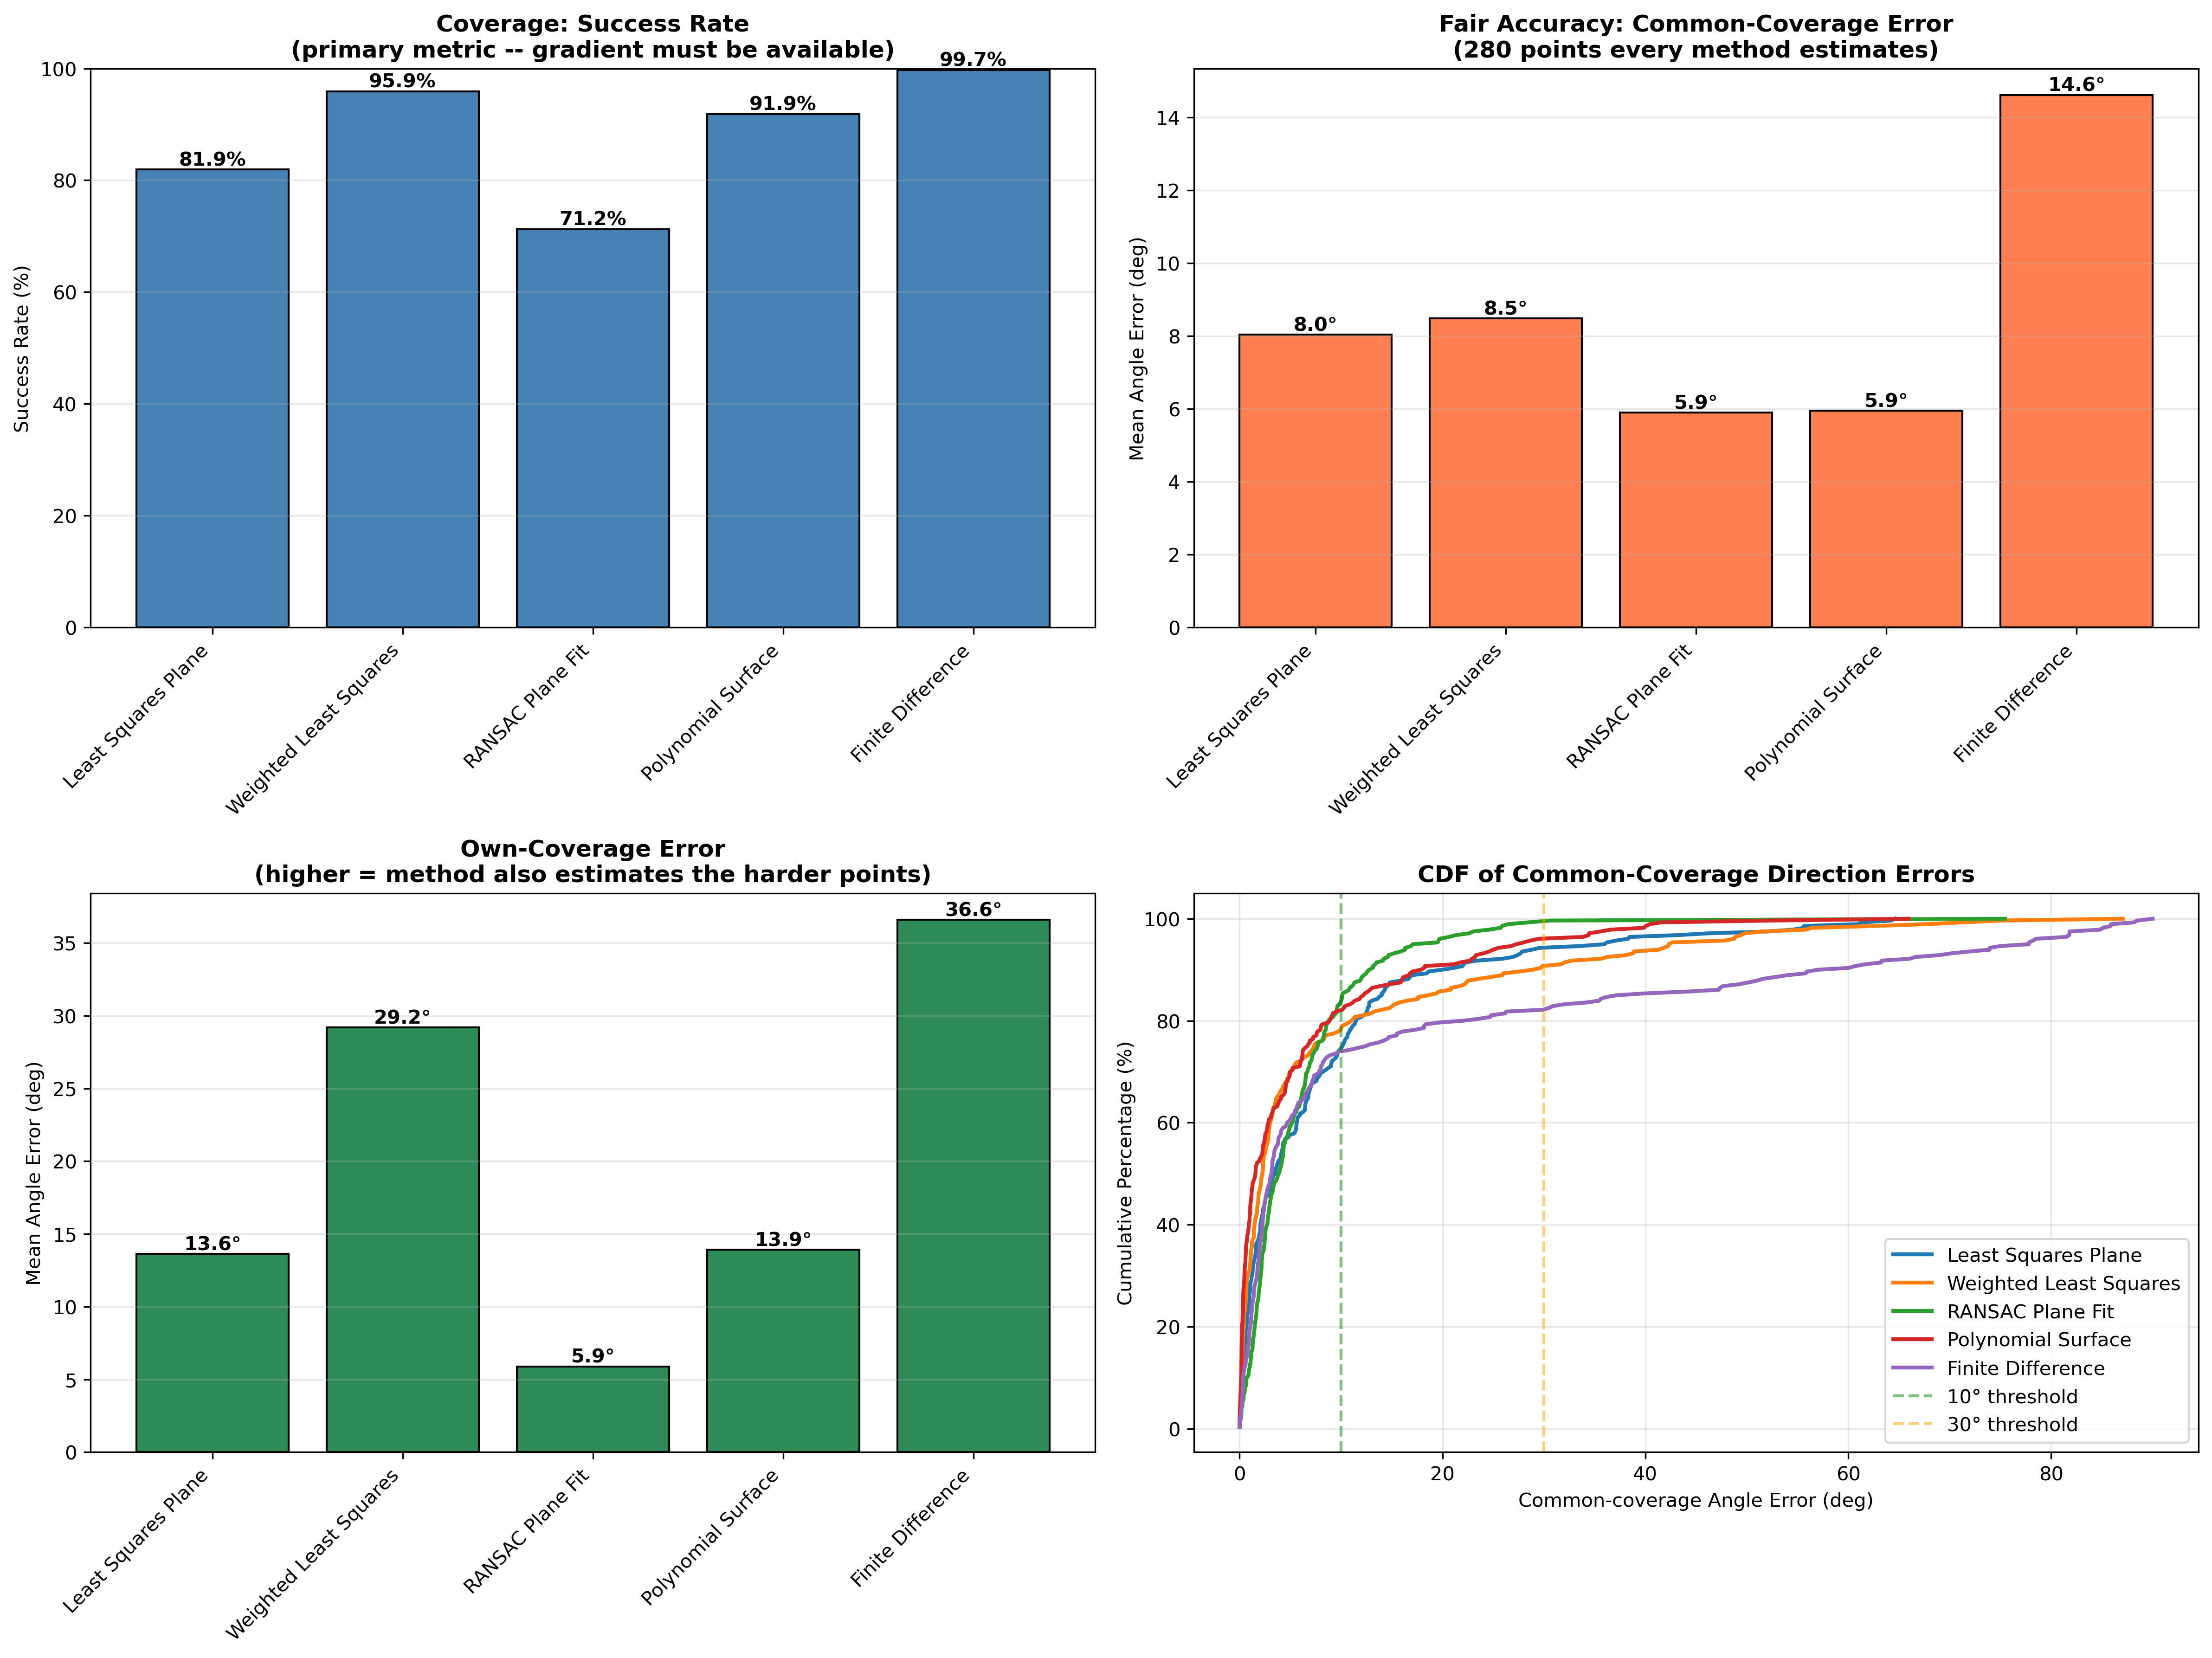
\includegraphics[width=0.85\textwidth]{figures/gradient_analysis/gradient_method_performance.png}
    \caption{Coverage and accuracy of the five gradient estimation methods on the reference map. Success rate is the share of points where the method returns a usable estimate. Accuracy is the angular error against the straight-to-source direction, reported both on the common set of points that every method estimates and on each method's own coverage.}
    \label{fig:gradient-comparison}
\end{figure}

Coverage is the criterion that matters most. The bearing already gives the
controller an accurate heading in open space, so the gradient 
does not have to be precise there; its job \hlnotein{is to be available wherever 
the drone is}{This needs to be rephrase. what does it mean wherever the drone is? I would
expect to read instead its improtant for drone to estimate the obstacle from the environment
at its current position. Have the ability to response at its current estimated location}, 
and above all when the bearing is lost behind an obstacle or 
between beacons. \hlnotein{A method that often returns nothing leaves the controller flying 
blind at exactly those moments.}{Also a bit confusing about what does this conveying. give
more specific example for context} \hlnote{Finite differences}{Add a method or algorithm behind
this so people know you are refering to previous several choices} return an estimate almost always,
at \hlnote{99.7\%}{What is this number meaning? Again this indicating the coverage needs
to be explain in a more easy way to understand}, but from so few cells that the 
direction is noisy; RANSAC succeeds least often, at 71\%, discarding too many cells 
as outliers; and the plane and polynomial fits sit between. Weighted least 
squares returns a usable estimate 96\% of \hlnotein{the time, second only to the 
noisy finite differences.}{I like the inspection and the analysis you tried to do here
But this really needs to rewrite. I will speak to you in detail to understand this part more}

The raw angular error, by contrast, is a misleading way to rank the 
methods, because it is entangled with coverage. A method that 
quietly fails on the hardest cells is never charged for them, 
so its average error flatters it, while a high-coverage method like 
weighted least squares is scored everywhere, including the cells right
under the elevated source where the measured field bends sharply
and behind the pillar where it leads around the obstacle rather than
straight at it. This shows directly in the figures: on its own coverage
weighted least squares records a mean error of 29 degrees, against 5.6 degrees
for the low-coverage RANSAC fit. When we instead score every method on the
same common set of cells, the cells that all of them estimate, the gap nearly
closes. The plane, polynomial, RANSAC and weighted least-squares fits then 
agree to within about three degrees, from 5.6 to 8.5 degrees of mean error,
with only finite differences staying noticeably noisier at 14.6 degrees;
weighted least squares itself falls from 29 to 8.5 degrees, which shows
that most of its apparent inaccuracy was simply the price of estimating
the difficult cells the other methods decline. The remaining differences
of a few degrees are not decisive: the bearing compensates them in open
space, and the steep field under the source would not even appear in
flight, where the drone follows a partial map and never measures that
drop.

\hlnote{Too complex}{Its fine to dig into detail here. but we need a major
refine of this. I think we need to put subsection in this section to first talk
about the setup, which is done good at first. And then subsection about different
method. and then subsection detail about the critirion that you are interested in. 
And then last subsection we compare them}

\begin{figure}[p]
    \centering
    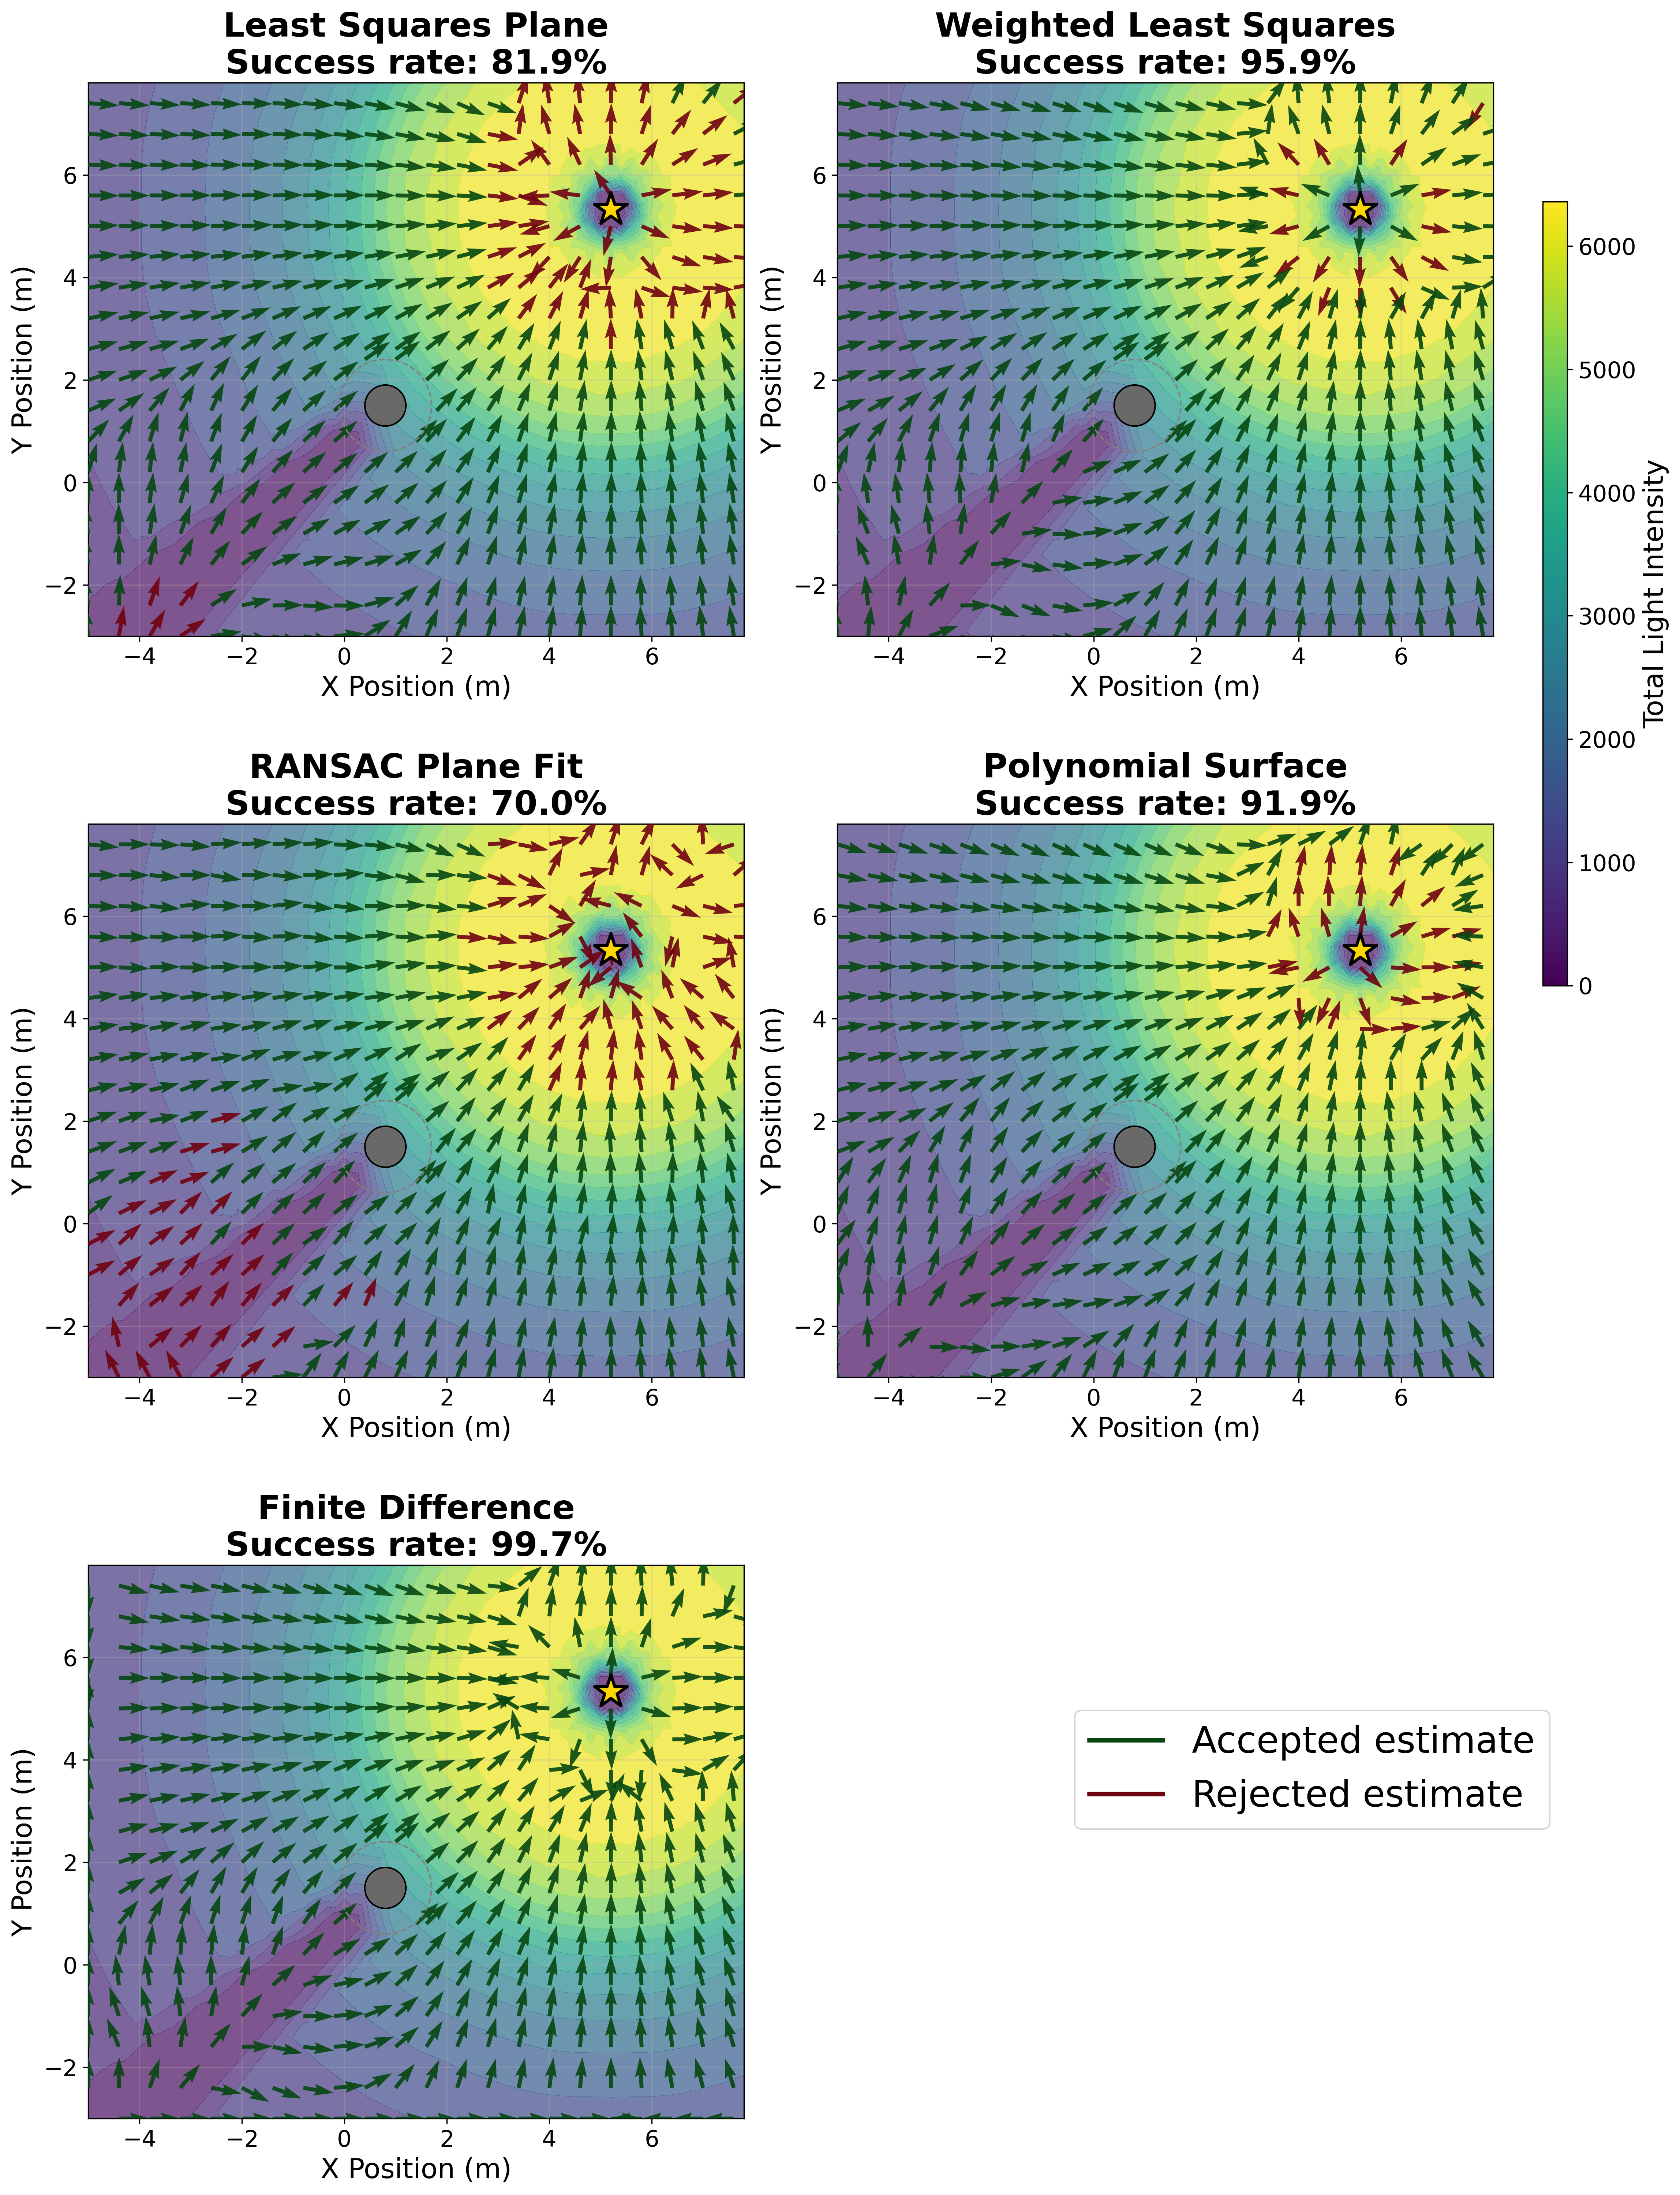
\includegraphics[height=0.86\textheight]{figures/gradient_analysis/gradient_method_comparison.png}
    \caption{Estimated gradient directions across the field for each method, coloured by angular error against the straight-to-source direction. The grey disc is the obstacle and the dashed circle the clearance the drone keeps. The large errors cluster under the source and behind the obstacle, where the field bends and pointing straight at the source is no longer the useful direction.}
    \label{fig:gradient-directions}
\end{figure}

Computational cost and robustness settle the choice. Weighted least squares 
solves one small fixed-size linear system whose runtime is the same on every call,
which sits comfortably within the budget of the drone's microcontroller, and its
inverse-distance weighting makes it robust to the changes in overall light level
that occur as the drone moves nearer to or further from the source. RANSAC, the
most accurate method on its own coverage, is the most expensive and the least
predictable, since it repeatedly fits and scores random subsets and its running
time varies from call to call, which is awkward for a real-time control loop on
a small processor. Finite differences are the cheapest but the noisiest.
Weighted least squares therefore offers the best combination for this platform:
the highest usable coverage, a low and constant computational cost, and
robustness to light-level changes, which is why the controller estimates
its gradient this way.

\section{Controller State Machine}

\hlnotein{A state machine governs what the drone does at each moment of a flight, 
since the bearing and gradient tell it which way to go but not what to do.}{1. state 
machine governs i understand 2. algorithm guide it where to go i understand. but what does 
it mean what to do?} It moves the drone through a small set of navigation phases, runs 
through them once for every beacon in the mission, and governs when the drone 
may rely on the map instead of the bearing, as Figure~\ref{fig:state-machine} \hlnotein{shows.}{
    again please clearly state the challenge first. here we should first write somthing like this.
    While combining the bearing angle and gradietn method can do something when it is exposed
    under sufficient light signal, when the light is block or simply out of field of view, or
    anything you come up with, the algorithm immediately fail. Second problem when drone is moving
    when do we need to trust the bearing and when is the gradient. list these problem first. and then
    bring up the state-machine to solve this
}

The drone starts in a searching phase, where it has no usable bearing or 
gradient yet. Here it slowly rotates in place to sweep the photodiode 
ring across the room until a beacon comes into view, and as soon as a
bearing arrives with enough signal strength to be trusted, the drone
moves on to aligning.

\hlnotein{In the aligning phase the drone turns toward the target without 
flying forward,}{So what we need to do here is first clarify what different stage is
and why? I know the graph might already show it. but we still need to write about it in
the context.} so that it is pointing roughly the right way before 
it commits to moving. Once its heading is within a small tolerance of 
the target it switches to approaching and begins to fly forward, correcting
its heading continuously as it goes. If it later drifts too far off heading,
it drops back to aligning.

Throughout aligning and approaching, the heading the drone follows 
is not the bearing alone. \hlnotein{While the map is still sparse the drone steers by 
the bearing, but as soon as the gradient becomes reliable the controller 
blends it into the heading, so the drone is already using both inputs together
well before it would ever need to fall back on the map by itself.}{I feel like here
is some grammar issue. for example->While the map is stil..., but as soon as..., I feel
like we are trying to say two things here? Please split this sentence and give more detail}

\hlnotein{The drone knows it has arrived when the signal strength climbs above an arrival 
threshold}{Bring this up like this. While now the drone can successfully move to the 
target, the drone needs to determine whether it reaches the target. and then we talk about the threshold.
and what threshold here trying to say? again bring up the intensy will increase and thus we can use it}, 
which only happens 
close to the beacon. The arrival threshold can be
tuned for different beacons or circumstances. It then enters a dwelling phase,
holding its position for a short, configurable time before moving on to the
next beacon and starting the cycle again. When the last beacon has been reached,
the mission is complete.

\hlnotein{The recovering phase is what keeps the drone moving when the beacon disappears, 
for example}{bring the example first, and then say we need the revoering} when 
an obstacle comes between the drone and the light and a purely 
\hlnotein{reactive controller would be stuck}{hard to understand what do you mean
reactive and what is \textit{stuck}}. If the bearing is lost but the gradient map 
is still reliable, the drone enters this phase and keeps flying forward on the 
gradient direction alone, climbing the stored light field to work its way out of 
the shadow. As soon as the beacon comes back into view it returns to approaching,
and only if the map itself becomes unreliable does it fall back to searching.

\begin{figure}[h]
    \centering
    \resizebox{\textwidth}{!}{%
    \begin{tikzpicture}[
        >=Latex,
        st/.style={draw, rounded corners, align=center, minimum height=8mm,
                   minimum width=20mm, inner sep=3pt, font=\small},
        lbl/.style={font=\scriptsize, align=center}
    ]
        \node[st] (S)  at (0,0)     {Searching};
        \node[st] (AL) at (3.6,0)   {Aligning};
        \node[st] (AP) at (7.4,0)   {Approaching};
        \node[st] (DW) at (11.0,0)  {Dwelling};
        \node[st] (RE) at (7.4,-2.5){Recovering};

        \coordinate (start) at (-1.8,0);
        \draw[->] (start) -- (S);

        \draw[->] (S) -- (AL) node[midway,above,lbl]{bearing\\acquired};
        \draw[->] (AL) to[bend left=18] node[midway,above,lbl]{aligned} (AP);
        \draw[->] (AP) to[bend left=18] node[midway,below,lbl]{off heading} (AL);
        \draw[->] (AP) -- (DW) node[midway,above,lbl]{arrived};
        \draw[->] (AP) to[bend left=12] node[midway,right,lbl]{signal lost} (RE);
        \draw[->] (RE) to[bend left=12] node[midway,left,lbl]{signal back} (AP);
        \draw[->] (RE) -- (S) node[midway,below,lbl,sloped]{map lost};
        \draw[->] (DW) to[bend right=22] node[midway,below,lbl]{next beacon} (S);
    \end{tikzpicture}}
    \caption{Navigation state machine, run once per beacon. The drone searches for the beacon, aligns its heading, then approaches while correcting; it dwells briefly on arrival before moving to the next beacon, and enters recovering to follow the gradient map alone when the bearing is lost behind an obstacle.}
    \label{fig:state-machine}
\end{figure}

\section{Control Output}

The controller's main output is a single target heading, formed by merging the 
bearing direction $\psi_B$ and the gradient direction $\psi_G$. Because both are angles,
we combine them with a weighted circular mean~\cite{mardia2000directional},
\begin{equation}
\psi = \operatorname{atan2}\!\big(w_B \sin\psi_B + w_G \sin\psi_G,\; w_B \cos\psi_B + w_G \cos\psi_G\big),
\label{eq:fusion}
\end{equation}
rather than a \hlnotein{plain average, which would suffer wrap-around errors near 
0 and 360 degrees.}{What does it mean wrap-around errors?} \hlnotein{When both inputs are 
reliable we set $w_B = w_G$, weighting }{Lets break this into more detail. So list several
case that is possible \textit{first} and then how we do corresponding to it.}
them equally; when only one is available its weight is one and the other zero; 
and when neither is, the drone holds its current heading. With these fixed, 
equal weights the combination is closer to a gated hand-off than to a continuous,
confidence-weighted fusion: where both signals overlap the heading is simply their
bisector, and the rest of the time the controller acts on whichever signal the
state machine deems reliable, the bearing in open space and the gradient behind
an obstacle. We keep this simple and predictable form here; letting $w_B$ and $w_G$
scale with a per-signal confidence is a natural extension we leave to future work.

\hlnotein{Alongside the heading, the controller sets a forward speed. The drone only flies
forward once it is roughly pointing at the target, so the speed is held
at zero while it is still turning to align and set to a fixed cruising 
speed once it is aligned and approaching. This keeps the drone from 
drifting sideways while it corrects a large heading error.

The heading and speed are handed to the drone's own flight controller
as setpoints, while the altitude is held at a fixed height throughout.
The controller therefore commands the drone in the horizontal plane only,
leaving the low-level work of stabilising the drone and holding altitude 
to the flight controller beneath it.}{Things like this can be shorten. since people
dont know what do you mean \textit{low-level}. discribing it like a simple robot.
what we are doing here is we want to find the best heading. thus we tried to dixed
the speed for the drone and the height is also predetermine. We can mentioned things like
horizontal plan only but what is the insight about this? probably the bad side? 
we need to bring up \textit{Why we want to mention it here?} if its hard to explain or
too long, just make it simple}
